\documentclass[10pt]{article}% uses letterpaper by default


%---------- Uncomment one of them ------------------------------
\usepackage[includeheadfoot, top=1in, bottom=1in, hmargin=1in]{geometry}

% \usepackage[a5paper, landscape, twocolumn, twoside,
%    left=2cm, hmarginratio=2:1, includemp, marginparwidth=43pt,
%    bottom=1cm, foot=.7cm, includefoot, textheight=11cm, heightrounded,
%    columnsep=1cm, dvips,  verbose]{geometry}
%---------------------------------------------------------------
\usepackage{fancyhdr}
%\usepackage{deluxetable}
\usepackage{verbatim}
\usepackage{url}
\usepackage{graphicx}
\usepackage{setspace}
\usepackage{wrapfig}
\usepackage{pdfpages}
\pagestyle{fancy}
\doublespacing
%\singlespacing
\onehalfspacing
\newcommand{\exercisename}{}


\rhead{Astronomy Lab}
\lhead{Spring 2013}
\lfoot{\large{J. Liu}} \cfoot{\thepage}

\renewcommand{\rightmark}{}
\newcommand{\degrees}{\ensuremath{^\circ}}
\newcommand{\arcmin}{\ensuremath{'}}
\newcommand{\arcsec}{\ensuremath{"}}
\newcommand{\hours}{\ensuremath{^\mathrm{h}}}
\newcommand{\minutes}{\ensuremath{^\mathrm{m}}}
\newcommand{\seconds}{\ensuremath{^\mathrm{s}}}

\begin{document}
\begin{center}

\huge\textbf{Measuring the Sky}
\end{center}

\begin{wrapfigure}{r} {0.35\textwidth}
\vspace{-10pt}
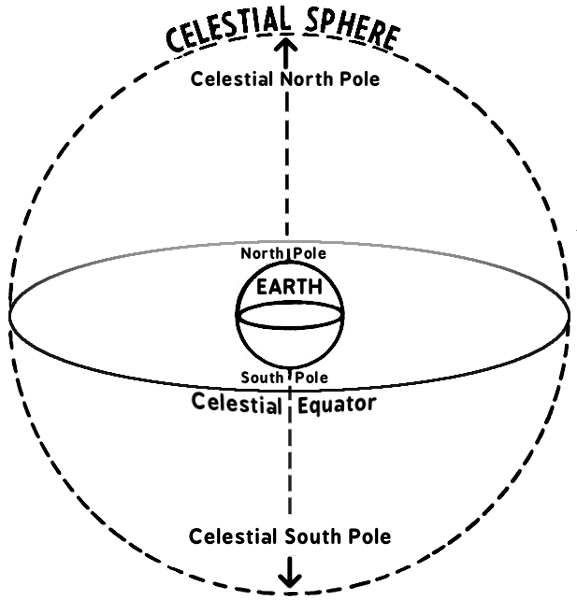
\includegraphics[scale=.32]{Celestial_sphere.png}
\vspace{-10pt}
\end{wrapfigure}

\section{Equatorial coordinate system}

On Earth, we can use longitude and latitude to specify the location of a place. Similarly, we use Right Ascension (RA, analogous to longitude) and Declination (DEC, analogous to latitude) to specify the celestial bodies. 

The celestial sphere is an imaginary hollow sphere centered on Earth, with an arbitrarily large radius. Its poles are aligned with the Earth's poles, as shown in the figure at right. 

DEC is measured in degrees, north or south of the celestial equator. The North and South celestial poles have DECs of +90 and -90 degrees, respectively. The equator has DEC 0.

RA is usually measured in hours, minutes and seconds (unlike longitude measured in degrees) in the east-west direction.  It ranges from 0$^{\rm \,h}$ to 23$^{\rm \,h}$ 59$^{\rm \,m}$ 59$^{\rm \,s}$.
\begin{equation}
{\rm \,RA (degrees)} = {\rm \,hours} \times 15 + {\rm \,minutes}/4 + {\rm \,seconds}/240.
\end{equation}

\begin{enumerate}
%\item If you stand in New York City and point to the upward vertical direction, the equatorial coordinate you point at is constantly changing due to the Earth's rotation. In this case, is DEC changing? Is RA changing? Why?

\item If you point your camera at Polaris and expose for the whole night, will Polaris move in your image? How about other stars?
%%% TA: polaris will stay pretty much still while other star form a circle, like e.g. http://www.koenvangorp.be/photos/2007_09_11-polaris_1500.jpg

\item Convert RA = 01$^{\rm \,h}$ 30$^{\rm \,m}$ 25$^{\rm \,s}$ to degrees.
%%% TA: 1.0*15+30.0/4+25.0/240 = 22.6 degrees
\end{enumerate}


\section{Planisphere}

In this section, you will learn to use planisphere, an astronomical observing tool refined in Greece during the 4th century by Hypatia, a notable mathematician and astronomer of her day.

On a planisphere, the brightness of a star is represented by the size of its dot. Usually a few dot sizes are used on the star map, each corresponding to a different range of brightness (magnitude). 

\begin{enumerate}
%\item What happens to the number of stars you see of a given brightness as you consider dimmer and dimmer magnitudes? Why does the star count depend on brightness like this? To simplify this problem, assume for a minute that all stars give off the same amount of light. Draw a diagram if you think it will aid your explanation.

%%% TA: the above question is normallly too difficult for student to answer.

\item Five of the planets in the sky are bright enough to outshine a lot of stars shown on the planisphere. Why aren’t the planets mapped? Hint: the word ``planet'' is derived from the Greek word for ``wandere''.
%%% TA: because planets moves thoughout the night.

\item Dial in the current time by aligning the date and time. What are the names of three bright stars (or the constellations they are in) overhead now?
%%% TA: for the time of the class, pick out the brightest ones on the planisphere.

\item Use your planisphere to answer this question. If it is currently midnight in New York, and you see Merak and Dubhe (the two starts in Ursa Major/the Big Dipper that are shown in the diagram below) pointing down vertically at Polaris. What month is it?
%%% TA: It's March (but you should check). What you need to do is rotate the planishpere to the configuration where Merak & Dubhe pointing down at polaris, and align that line with 12AM. And see which month it falls onto. From this question, students should learn to: 1) orient the planisphere to match the sky; 2) find stars on the planishpere; 3) certain combination of time & date gives a specific sky configuration.

\item BTW, if you are interested to observe the night sky out of the class (not required), you can use the last 2 pages of this lab to make your own planisphere!
%%% TA: nothing to be done here.
\end{enumerate}

\begin{center}
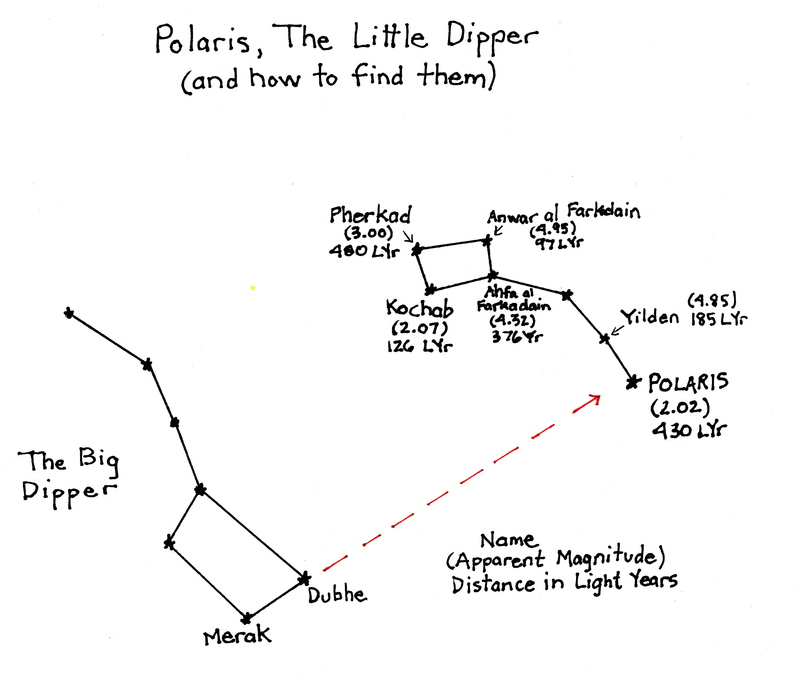
\includegraphics[scale=1.5]{little-dipper.jpg}
\end{center}



\section {Use your thumb and fist as measuring tools}

\begin{center}
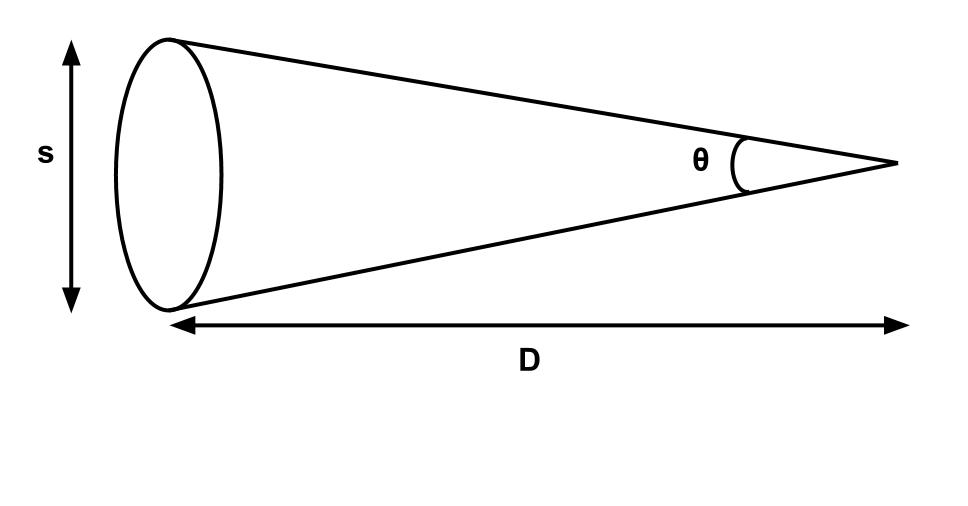
\includegraphics[scale=0.25]{angularsize.jpg}
\vspace{-14pt}
\end{center}

\begin{enumerate}

\item Measure the width of your thumb (across the nail) , and measure the length of your arm (from your eyes to the thumb). Use these measurements to determine the angular size ($\theta$) of your thumb in degrees when you hold it up straight forward.
\begin{equation}
{\rm \,\theta (degrees)} = 360\times({\rm \,s/D})
\end{equation}
where s is the width of your thumb, and D is the length of your arm. (hint: you should get something like 1 degree).

\item Now do the same for your fist (across the knuckles). What is the angular size of your fist when you hold it up straight forward? (hint: you should get something like 5-10 degrees)
%%% TA: students normally take a long time to calibrate these 2 angles, so to accelerate the process, tell them clearly there are only 3 measurements: thumb, fist, and length of arm. And use the equation to get answer.

%\item Have one person stand away. Hold your fist straight away from you, and then move your relative position until your fist covers your view of the person. Approximately how far away is the person? (use the degree information you just measured). Compare your answer with the actual distance (use a meter stick).
%%% TA: I expect this to be too long so only uncomment this question if you think your lab will do this fast.

\end{enumerate}

\section{Outdoor part}

\begin{enumerate}
\item With your planisphere, orient yourself and identify as many constellations as you can from the roof. Write them down in your notebook.

\item Pick two stars that are close to the celestial equator (90 degrees away from Polaris), and pick a stationary object on Earth that is also close to the celestial equator (tree, building, etc.). 

To find celestial equator, point your right arm towards Polaris, and point your left arm towards some stars. Make your two arms form a right angle, the circle that your left arm can point to is the celestial equator.

Measure distances from each star to the stationary object in degrees with your fist and/or thumb. Note the time. Do the same measurement again in 30 minutes (while waiting for the second measurement, you can proceed to the next task). Write down the distances and time of measurement.

Derive the Earth's rotation (in degrees/hour) from the measurements. Compare this value from the actual value (15 degrees/hour). % What is your fractional difference (~$|$measured value/actual value~-~1$|$~ )?

\item Measure the angle from the horizon to Polaris. Draw a diagram and explain how you can use your measured angle to calculate the latitude of New York City.

\item Find the following objects using the telescope: Rigel (Beta Orionis, blue supergiant and double star in Orion), Betelgeuse (Alpha Orionis, red supergiant in Orion), M 34 (open cluster of more than 20 stars, in the constellation Perseus). Show them to your TA.
%%% TA: the objects are likely to change month by month, please change accordingly.

%%% Feb/Mar: Rigel (Beta Orionis, blue supergiant and double star in Orion), Betelgeuse (Alpha Orionis, red supergiant in Orion), M 34 (open cluster of more than 20 stars, in the constellation Perseus).

%%% April: Beehive Cluster (M44, open star cluster with approximately 100 stars, in the constellation Cancer), Whirlpool Galaxy (M51, face-on spiral galaxy with interacting companion, in the constellation Canes Venatici), M3 (globular cluster, in the constellation of Canes Venatici).

%%% May: Whirlpool Galaxy (M51, face-on spiral galaxy with interacting companion, in the constellation Canes Venatici), M3 (globular cluster, in the constellation of Canes Venatici), Mizar & Alcor (Bright double star, easy to find in Big Dipper).

% optional \item To measure the Earth's rotation more accurately, we now look at the stars through the telescope. Point the telescope towards a star near the celestial equator. Position the target at the eyepiece.

% Draw a circle in your notebook showing the field of view and the star's position in it, note the time. Keep observing the star's movement in the eye piece, and write down corresponding time, until the star entirely disappears from view. From the previous measurement, you already know that the Earth's rotation is 15 degrees per hour. Using equation 1, derive the field of view of the eye piece in degrees.

%%% TA: answer: 15 * t, where t is the time takes the star moves from one side to another side of the eyepiece. We're likely to use the small dome for this question, since the dops are too shaky, but I don't know the exact answer to it.

\end{enumerate}



\includepdf[pages={1,2},angle=90]{planisphere-e.pdf}
\end{document}